\section{Algebraic Moment Closures}
\label{sec:algebraicClosure}

The two-moment model given by Eq.~\eqref{eq:angularMoments} is not closed because of the appearance of the second moments $\vect{\cK}$ (the normalized pressure tensor).  
Algebraic moment closures for the two-moment model are computationally efficient as they provide the Eddington factor in Eq.~\eqref{eq:eddingtonTensor} in closed form as a function of the density $\cJ$ and the flux factor $h=|\vect{\cH}|/\cJ$.  
For this reason they are widely used in applications where radiation transport plays an important role --- including simulation of neutrino transport in core-collapse supernovae \cite{roberts_etal_2016} and compact binary mergers \cite{foucart_etal_2015}.  
Algebraic moment closures in the context of these aforementioned applications have also been discussed elsewhere (e.g., \cite{pons_etal_2000,smit_etal_2000,just_etal_2015,murchikova_etal_2017}).  
The family of algebraic closures we consider in this paper can be written in the form \cite{cernohorskyBludman_1994}
\begin{equation}
  \chi(\cJ,h)=\f{1}{3}+\f{2\,(1-\cJ)\,(1-2\cJ)}{3}\,\Theta\Big(\f{h}{1-\cJ}\Big),
  \label{eq:eddingtonFactor}
\end{equation}
where the \emph{closure function} $\Theta(x)$ varies with the specifics of the closure procedure.  
We will consider two basic closure procedures in more detail below: the maximum entropy (ME) closure and the Kershaw (K) closure.  

\paragraph{Low Occupancy Limit}
We note in passing that in the low occupancy limit ($\cJ\ll1$), the Eddington factor in Eq.~\eqref{eq:eddingtonFactor} depends solely on $h$; i.e.,
\begin{equation}
  \chi(\cJ,h)\to\chi_{0}(h)=\f{1}{3}+\f{2}{3}\,\Theta\big(h\big).  
  \label{eq:eddingtonFactorLow}
\end{equation}
This is also a form of algebraic moment closure suitable for particle systems obeying Maxwell-Boltzmann statistics.  

\subsection{Maximum Entropy (ME) Closure}

For the two-moment model, the ME closure constructs the least biased angular distribution based on the limited information available (i.e., $\cJ$ and $\vect{\cH}$) \cite{cernohorskyBludman_1994,lareckiBanach_2011}.  
The ME distribution $f_{\mbox{\tiny ME}}(\omega)$ is found by maximizing the entropy functional, which for particles obeying Fermi-Dirac statistics is given by
\begin{equation}
  S[f_{\mbox{\tiny ME}}] 
  = \int_{\bbS^{2}}\big[\,(1-f_{\mbox{\tiny ME}})\log(1-f_{\mbox{\tiny ME}}) + f_{\mbox{\tiny ME}}\log f_{\mbox{\tiny ME}}\,]\,d\omega,
  \label{eq:entropyFunctional}
\end{equation} 
subject to the constraints
\begin{equation}
  \f{1}{4\pi}\int_{\bbS^{2}}f_{\mbox{\tiny ME}}(\omega)\,d\omega=\cJ
  \quad\text{and}\quad
  \f{1}{4\pi}\int_{\bbS^{2}}f_{\mbox{\tiny ME}}(\omega)\,\vect{\ell}(\omega)\,d\omega=\vect{\cH}.  
  \label{eq:closureConstraints}
\end{equation}
From the variation of the entropy functional in Eq.~\eqref{eq:entropyFunctional} with respect to $f_{\mbox{\tiny ME}}$, and introducing Lagrange multipliers ($a$ and $\vect{b}$) to enforce the constraints in Eq.~\eqref{eq:closureConstraints}, the ME distribution takes the general form
\begin{equation}
  f_{\mbox{\tiny ME}}(\omega;a,\vect{b})=\f{1}{e^{a + \vect{b}\cdot\vect{\ell}(\omega)}+1}.  
  \label{eq:fME}
\end{equation}
The Lagrange multipliers are implicit functions of $\cJ$ and $\vect{\cH}$.  
The ME distribution function satisfies $0 \le f_{\mbox{\tiny ME}} \le 1$, but $a$ and $\vect{b}$ are unconstrained.  
Specification of $a$ and $\vect{b}$ from $\vect{\cM}=(\cJ,\vect{\cH})^{T}$ gives $f_{\mbox{\tiny ME}}$, and any number of moments can in principle be computed.  
Importantly, we note that for the maximum entropy problem to be soluble, we must have $\vect{\cM}\in\cR$ \cite{lareckiBanach_2011}.  

To arrive at the algebraic form of the ME closure, Chernohorsky \& Bludman \cite{cernohorskyBludman_1994} postulate (but see \cite{lareckiBanach_2011}) that, as a function of the so-called flux saturation $x=h/(1-\cJ)$, the closure function $\Theta(x)$ is independent of $\cJ$ and can be written explicitly in terms of the inverse Langevin function.  
To avoid inverting the Langevin function for $\Theta(x)$, they provide a polynomial fit (accurate to $2\%$) given by
\begin{equation}
  \Theta_{\mbox{\tiny ME}}^{\mbox{\tiny CB}}(x)
  =\f{1}{5}\,\big(\,3-x+3\,x^{2}\,\big)\,x^{2}.
  \label{eq:closureMECB}
\end{equation}
More recently, Larecki \& Banach \cite{lareckiBanach_2011} have shown that the explicit expression given in \cite{cernohorskyBludman_1994} is not exact, and provide another approximate expression
\begin{equation}
  \Theta_{\mbox{\tiny ME}}^{\mbox{\tiny BL}}(x)
  =\f{1}{8}\,\big(\,9\,x^{2}-5+\sqrt{33\,x^{4}-42\,x^{2}+25}\,\big),
  \label{eq:closureMEBL}
\end{equation}
which is accurate to within $0.35\%$.  
On the interval $x\in[0,1]$, the curves given by Eqs.~\eqref{eq:closureMECB} and \eqref{eq:closureMEBL} lie practically on top of each other.  
The closure functions given by Eqs.~\eqref{eq:closureMECB} and \eqref{eq:closureMEBL}, together with the Eddington factor in Eq.~\eqref{eq:eddingtonFactor} and the pressure tensor in Eq~\eqref{eq:eddingtonTensor}, constitute the algebraic maximum entropy closures for fermionic particle systems considered in this paper.  
We will refer to the ME closures with $\Theta_{\mbox{\tiny ME}}^{\mbox{\tiny CB}}$ and $\Theta_{\mbox{\tiny ME}}^{\mbox{\tiny BL}}$ as the CB (Cernohorsky \& Bludman) and BL (Banach \& Larecki) closures, respectively.  

We also note that using the closure function given by Eq.~\eqref{eq:closureMECB} with the low occupancy Eddington factor in Eq~\eqref{eq:eddingtonFactorLow} results in the algebraic maximum entropy closure attributed to Minerbo \cite{minerbo_1978}, which is currently in widespread use in simulation of neutrino (fermion) transport in the aforementioned nuclear astrophysics applications.  
In a recent comparison of algebraic (or analytic) closures for the two-moment model applied to neutrino transport around proto-neutron stars, Murchikova et al. \cite{murchikova_etal_2017} obtained nearly identical results when using the closures of CB and Minerbo.  
For these reasons, we include the Minerbo closure in the subsequent discussion and in the numerical tests in Section~\ref{sec:numerical}.  

\subsection{Kershaw (K) Closure}

The basic principle behind Kershaw closure is derived from the fact that the realizable set defined by $(\cJ, \vect{\cH}, \vect{K})$ is convex.
Due to the convexity, any element in the convex set be expressed as a convex combination of two elements that on the set boundary, and vice versa.
That is,
\begin{align}
 \chi(\cJ,h) = \beta  \chi_{L}(\cJ,h) + (1-\beta) \chi_{U}(\cJ,h),
\end{align}
with $\chi_{L}$ and $\chi_{U}$ be the boundary elements, and $\beta \in [0,1]$. 
The Kershaw closure uses a convex combination that determined by the isotropic distribution case to approximate $\chi(\cJ,h)$:
\begin{align}
 \chi(\cJ,0)  &= \dfrac{1}{3},\\
\chi_{L}(\cJ,h) & = \dfrac{1}{3}\cJ^2 + h^2, \\
\chi_{U}(\cJ,h) & = \left( 1 - \cJ + \dfrac{1}{3}\cJ^2 \right) - \dfrac{h^2 \cJ}{1-\cJ},
\end{align}
$\chi_{L}$ and $\chi_{U}$ are given by the Heaviside function with Fermi-Dirac statistic function, and
\begin{align}
\beta = \dfrac{2 - \cJ}{3}.
\end{align}
Then the Kershaw closure function $\Theta(x)$ reads (Banach \& Larecki \cite{banachLarecki_2017a}):
\begin{equation}
  \Theta_{\mbox{\tiny K}}^{\mbox{\tiny BL}}(x)=x^{2}
\end{equation}

\subsection{Realizability of Algebraic Moment Closures}

It is not immediately obvious that all the algebraic moment closures discussed above are suitable for the design of a realizability-preserving method for the two-moment model of fermion transport.  
In particular, the realizability-preserving scheme developed in this paper is based on the result in Lemma~\ref{lem:explicitStep}, which must hold for the adapted closure.  
The Kershaw closure is consistent with a bounded distribution, $f_{_{\mbox{\tiny K}}}\in[0,1]$, and should be well suited, but the algebraic ME closures are based on approximations to the closure function, and we must make sure that these approximate closures remain consistent with the assumed bounds on the underlying distribution function.  
To this end, we rely on results due to \cite{levermore_1984,lareckiBanach_2011} (see also \cite{kershaw_1976,shohatTamarkin_1943}):  Realizability of the moment triplet $\{\cJ,\vect{\cH},\vect{\cK}\}$ (i.e., they are consistent with a bounded distribution function $0 \le f<1$), with $\vect{\cM}=(\cJ,\vect{\cH})^{T}\in\cR$ and $\vect{\cK}$ given by Eq.~\eqref{eq:eddingtonTensor} is equivalent to the following requirement for the Eddington factor
\begin{equation}
  \chi_{\mbox{\tiny min}}
  =\max\big(1-\f{2}{3\cJ},h^{2}\big)
  <\chi<\min\big(1,\f{1}{3\cJ}-\f{\cJ}{1-\cJ}h^{2}\big)=\chi_{\mbox{\tiny max}}.  
\end{equation}
(Note that for $\cJ\ll1$ this limits to the bounds for positive distributions given by Levermore \cite{levermore_1984}: $h^{2}\le\chi\le1.$)

In Figure~\ref{}, we plot the Eddington factor $\chi$ versus the flux factor $h$ for the various algebraic closures discussed above for different values of $\cJ\in(0,1)$.  

Figure~\ref{fig:MabWithDifferentClosure} illustrates the behavior of these four closure.
As it shows, Minerbo closure (right bottom) is the only one among those four closures that does not preserve realizability.
\begin{figure}[h]
  \centering
  \begin{tabular}{cc}
    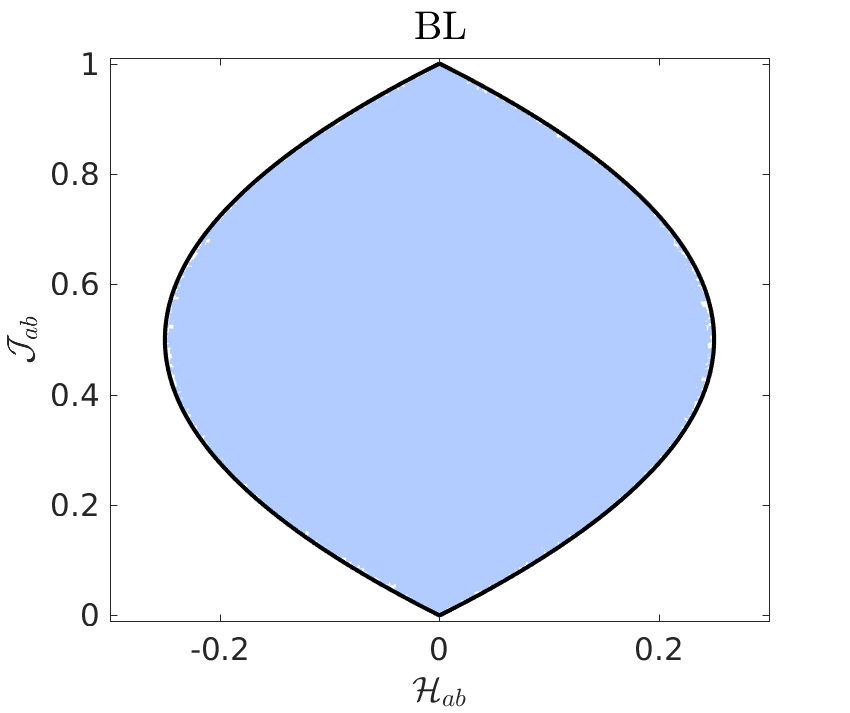
\includegraphics[width=0.5\textwidth]{figures/MabWithBLME}
    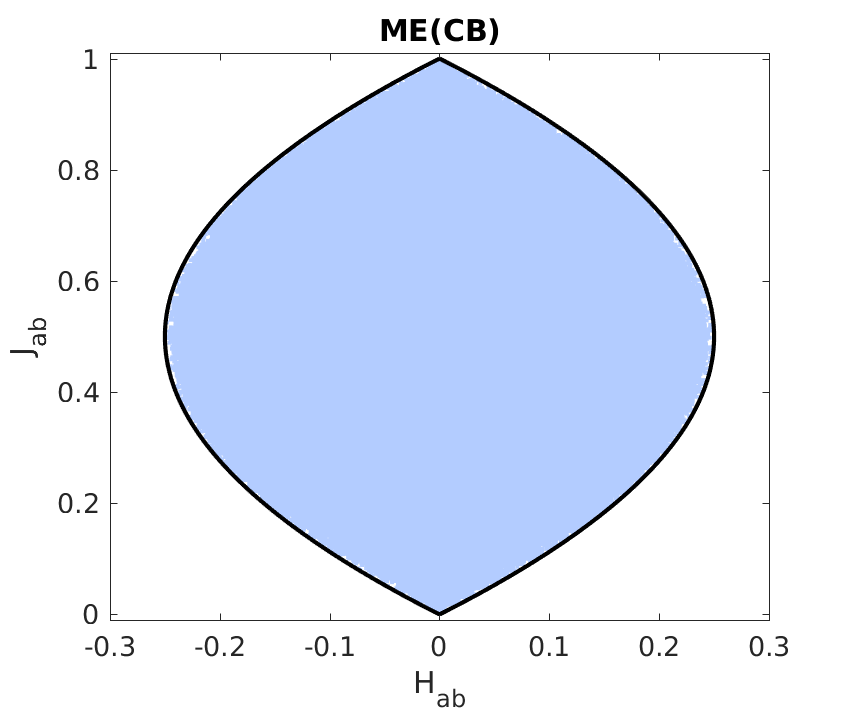
\includegraphics[width=0.5\textwidth]{figures/MabWithCBME} \\
    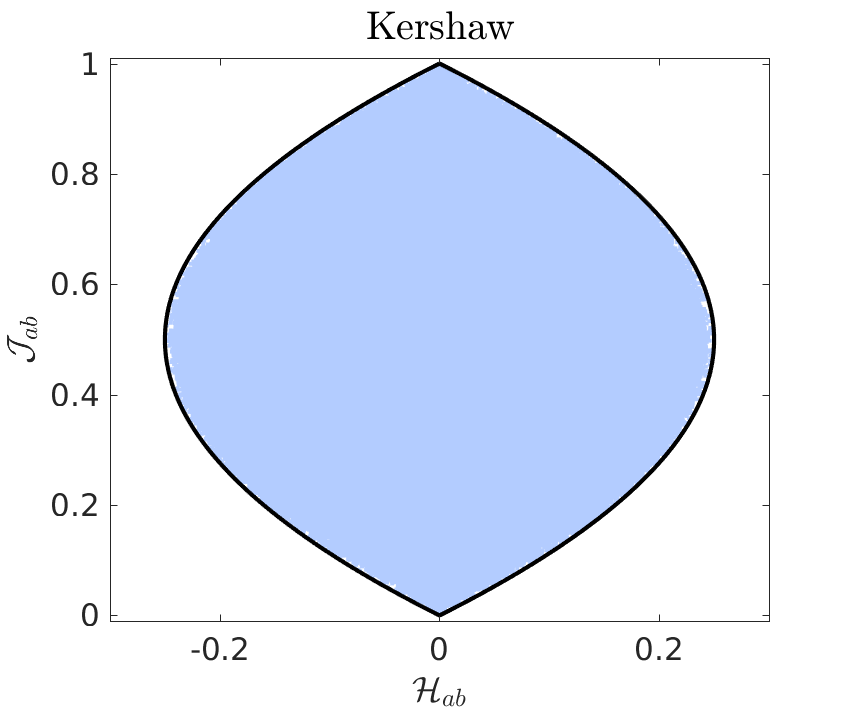
\includegraphics[width=0.5\textwidth]{figures/MabWithBLKS}
    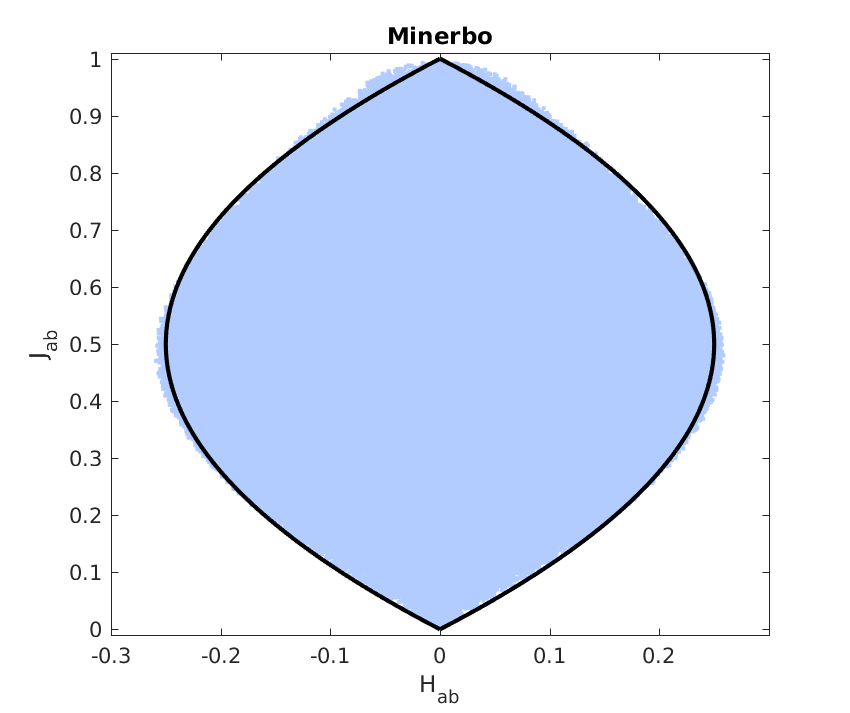
\includegraphics[width=0.5\textwidth]{figures/MabWithMI}
  \end{tabular}
   \caption{Illustration of $\vect{\cM}_{ab}$ with four different closures: Banach \& Larecki maximum entropy closure (left top), Chernohorsky \& Bludman maximum entropy closure (right top), Kershaw closure (left bottom), and Minerbo closure (right bottom).
   Total $10^{6}$ pairs of random Fermi-Dirac distribution were generated.
   With these pairs, $\vect{\cM}_{ab}$ with different closures were calculated separately and marked with light-blue points.
   Black lines define the boundary of $\cR$: $\gamma(\vect{\cM}) = 0$.}
  \label{fig:MabWithDifferentClosure}
\end{figure}